\chapter{Przegląd istniejących rozwiązań}
\label{cha:Przeglad_istniejacych_rozwiazan}

\todo{Więcej przykładów}

\section{Moduł sterowania kamerą \textit{pan-tilt} dla pojazdu \textit{UAV}}
\label{sec:Przyklad_Olivares-Mendez2009}

W publikacji \cite{Olivares-Mendez2009} przedstawiono system sterowania głowicą \textit{pan-tilt} z kamerą wizyjną, zamontowaną na pojeździe \textit{UAV} (rysunek \ref{fig:UAV_Olivares_Mendez}). Jak wskazują autorzy, w przypadku aplikacji tego typu, w kontekście śledzenia wizyjnej znacznym problemem jest połączenie zjawiska wibracji całego pojazdu i długiej ogniskowej kamery. Zastosowanie platformy \textit{pan-tilt} ułatwia śledzenie i wykrawanie obiektów zainteresowanie, nie wymaga bowiem zmiany orientacji całego pojazdu.
\begin{figure}[!htb]
	\begin{center}
		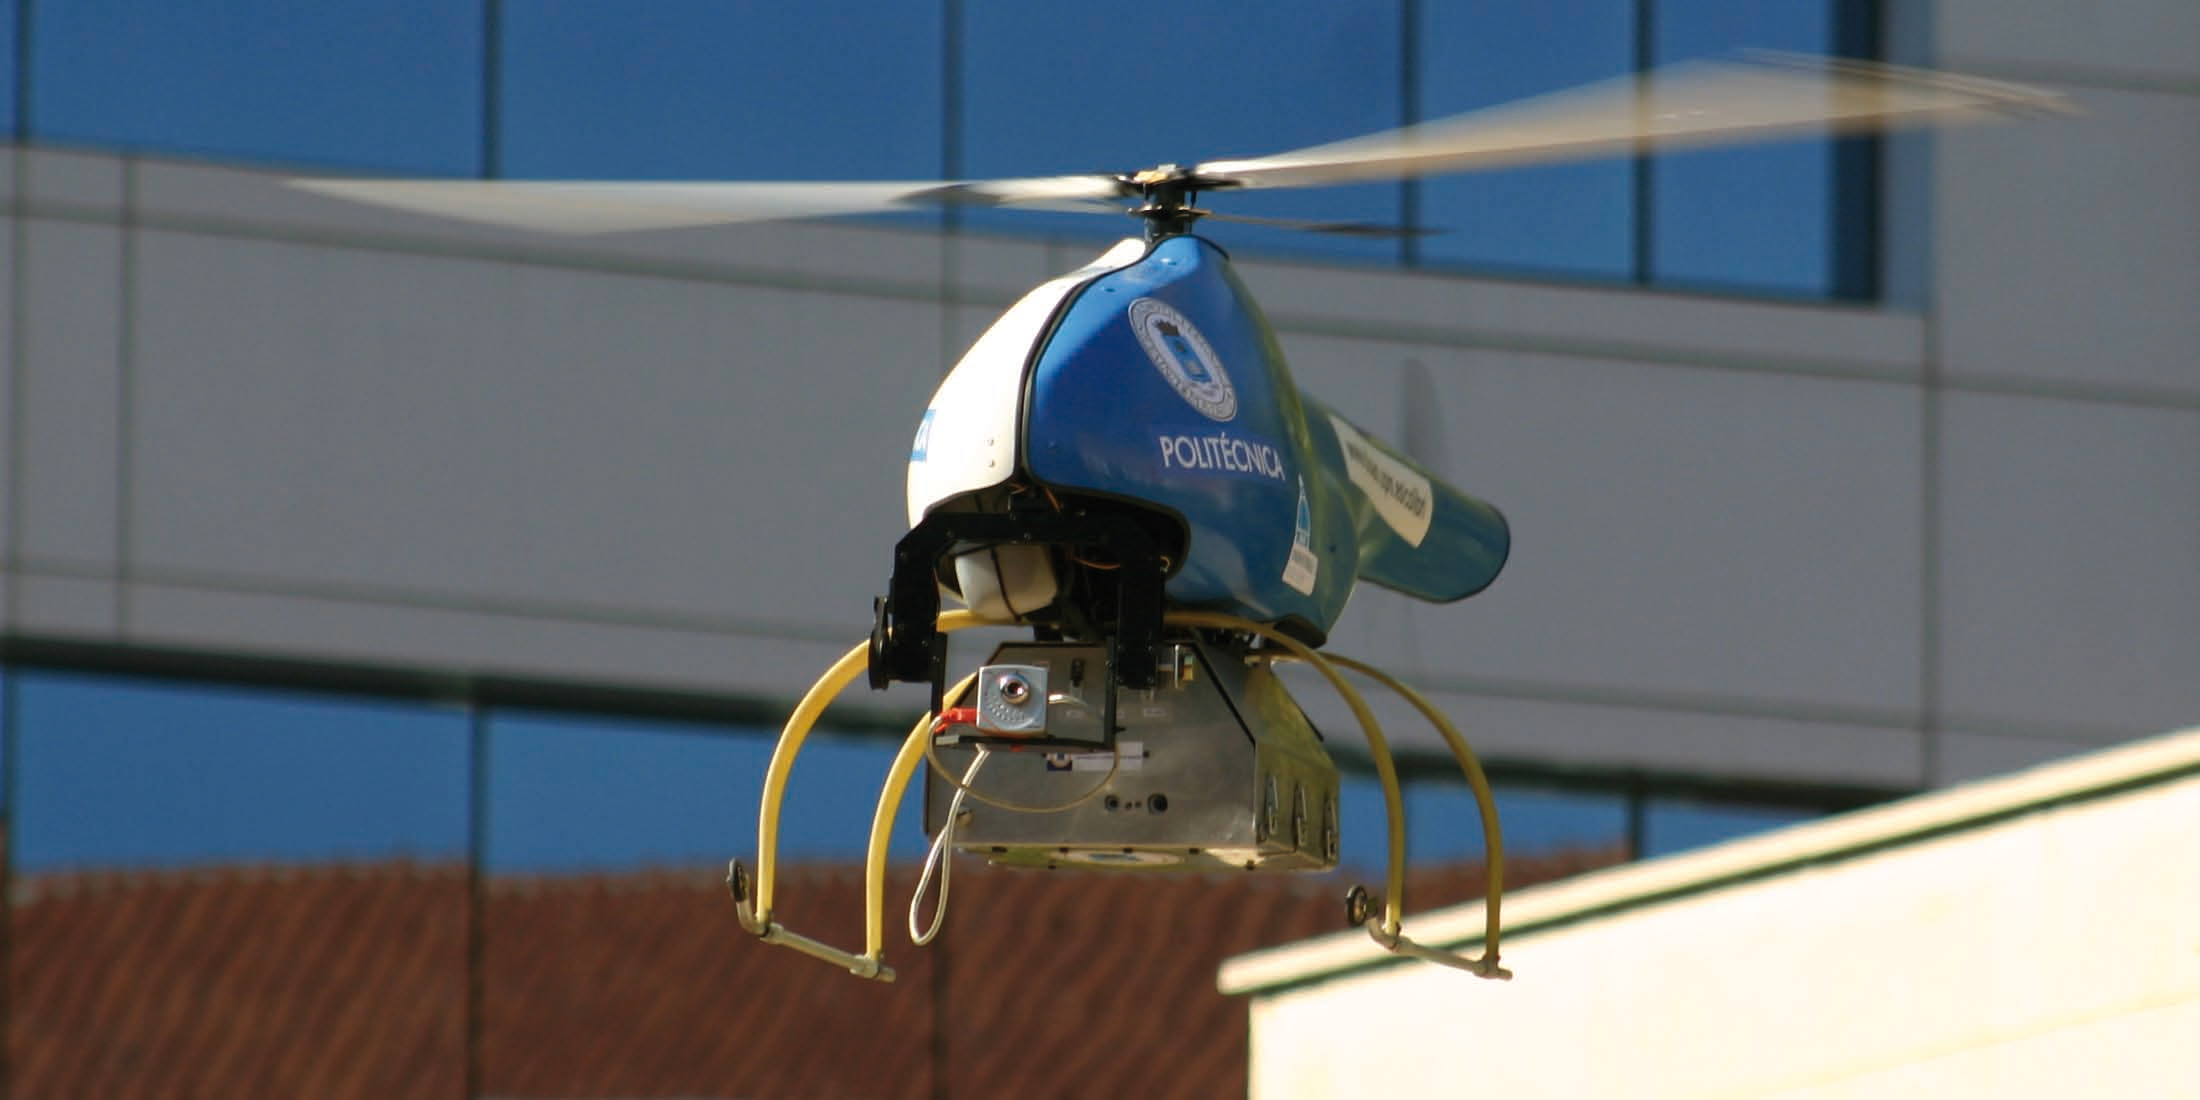
\includegraphics[width=12cm]{images/uav_olivares_mendez.png}
	\end{center}	
	\longcaptionsource{Bezzałogowy helikopter - platforma testowa}{}{\cite{Olivares-Mendez2009}}
\label{fig:UAV_Olivares_Mendez}
\end{figure}

Obiekt zainteresowania jest wykrywany przez system poprzez wykrawanie punktów zainteresowania według algorytmu Harrisa, w którym narzucono dodatkowo kryterium maksymalnej wariancji przy zwiększaniu okna wykrawania oraz minimalnego progu modułu wartości własnych. Pozwoliło to na wybranie punktów zainteresowania o największej odporności oraz wykorzystanie ich jako reprezentacji śledzonego obiektu w algorytmie Lucasa-Kanade (wersja klasyczna, opisana w rozdziale \ref{subsec:Klasyczny_algorytm_Lucasa_Kanade}).
Zwracany przez niego błąd śledzenia (rozbieżność pomiędzy położeniem obiektu a środkiem obrazu) wraz z różnicą pomiędzy jego bieżącą o poprzednią wartością stanowi sprzężenie zwrotne dla dwóch kontrolerów działających w oparciu o wnioskowanie rozmyte {ang. \textit{fuzzy controllers}), które sterują pracą silników obydwu osi platformy \textit{pan-tilt}. Wyjście kontrolerów stanowi względne przemieszczenie kątowe, które musi zostać wykonane w celu wycentrowania obiektu w polu widzenia kamery i jest wyznaczane na podstawie 49 zasad wnioskowania.

Działanie systemu zostało przetestowane przy wykorzystaniu pojedynczej kamery video o rozdzielczości $320 \times 240$ pikseli, środowiskiem działania był system Linux, zainstalowany na pokładowym komputerze VIA mini-ITX (częstotliwość taktowania 1,5GHz, 1Gb pamięci RAM).

\section{Hybrydowy algorytm śledzenia i podążania za ludźmi dla robota kroczącego}
\label{sec:Przyklad_Liem2008}

Celem autorów publikacji \cite{Liem2008} było opracowanie algorytmu śledzenia i podążania za ludźmi dla robota kroczącego, który umożliwiałby stały nadzór osób starszych, pacjentów szpitali, etc. Jako platformę testową wykorzystano robota Sony AIBO, wskazując na jego zalety w postaci wyposażenia w szereg sensorów (w tym kamerę video) oraz nierzucający się w oczy wygląd. Istotnym wymaganiem wobec opracowanego rozwiązania było osiągnięcie odporności na nieprzewidywalny i nieregularny ruch kamery, wynikający ze sposobu poruszania się robota, oraz zmian w oświetleniu obiektu zainteresowania.

Uproszczony przebieg algorytmu wizyjnego śledzenia obiektu przedstawiono na rysunku \ref{fig:Przebieg_algorytmu_Liem}. Wykrycie obiektu następuję poprzez segmentację tła i pierwszego planu (obiektów poruszających się) z wykorzystaniem metody \textit{Gaussian Mixture Model}. Następnie obiekt jest śledzony z wykorzystaniem algorytmu \textit{EM-Shift}, stanowiącego rozwinięcie metody \textit{Mean Shift} (rozdział \ref{subsec:Algorytm_Mean_Shift_w_sledzeniu_obiektow}), w którym dodatkowo wykonywana jest estymacja i adaptacja okna przeszukiwania. Obiekt jest również śledzony z wykorzystaniem algorytmu Lucasa-Kanade-Tomasi (rozdział \ref{subsec:Algorytm_Kanade_Lucasa_Tomasi}) i wyznaczonych według niego punktów zainteresowania. Krok początkowy (segmentacja poruszających się obiektów) nie może realizować bezpośrednio zadania śledzenia ze względu na możliwy ruch kamery. Algorytm \textit{EM-Shift} działa w oparciu o histogram obiektu zainteresowania, co w wypadku zmiany oświetlenia może prowadzić do zgubienia obiektu. Z kolei \textit{KLT} nie dokonuje segmentacji obiektu jako takiej, przez co nie można stwierdzić czy śledzone przez niego punkty faktycznie należą do obiektu. Połączenie tych dwóch metod śledzenia obiektów pozwala na kompensację ich wad i uzyskanie odpornego rozwiązania.
\begin{figure}[!htb]
	\begin{center}
		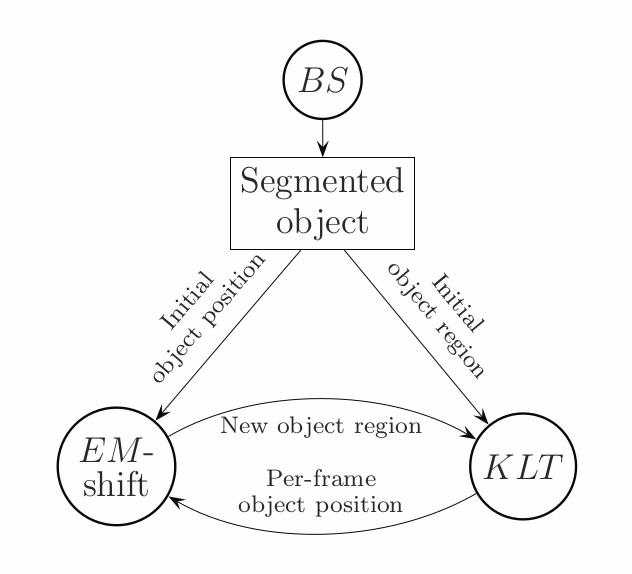
\includegraphics[width=6cm]{images/algorithm_liem.png}
	\end{center}	
	\longcaptionsource{Przebieg algorytmu wizyjnego śledzenia obiektu}{Od góry, od lewej: odejmowanie tła - segmentacja obiektu; algorytm \textit{EM-shift} - wykrywanie nowego obszaru zainteresowania; algorytm Lucasa-Kanade-Tomasi - wykrywanie nowych współrzędnych obiektu}{\cite{Liem2008}}
\label{fig:Przebieg_algorytmu_Liem}
\end{figure}

Pokładowa kamera robota ma rozdzielczość $208 \times 160$ pikseli, obliczenia w trakcie testów były wykonywane zdalnie, za pośrednictwem sieci WiFi, na komputerze PC z procesorem AMD 3500+ i 2Gb pamięci RAM.

\section{Algorytm wykrywania, śledzenia i podążania za obiektami na obrazie z kamery sferycznej dla robota mobilnego}
\label{sec:Przyklad_Markovic2014}

W pracy \cite{Markovic2014} zaprezentowano algorytm wykrywania, śledzenia i podążania za obiektami, którego czujnik wizyjny stanowi kamera sferyczna (ang. \textit{omnidirectional camera}), dostarczająca kompletnego obrazu sceny w promieniu {360\textdegree} (rysunek \ref{fig:Kamera_sferyczna_Markovic}). Przy zastosowaniu kamery tego typu nie istnieje możliwość ucieczki obiektu zainteresowania poza pole widzenia, w związku z tym system sterowania nie musi realizować funkcji utrzymywania go w centrum obrazu. Zakłada się jednoczesny ruch zarówno obiektu zainteresowania jaki i robota. Jako platformę testową wykorzystano robota kołowego Pioneer 3DX oraz kamerę z obiektywem typu \textit{fisheye}.
\begin{figure}[!htb]
	\begin{center}
		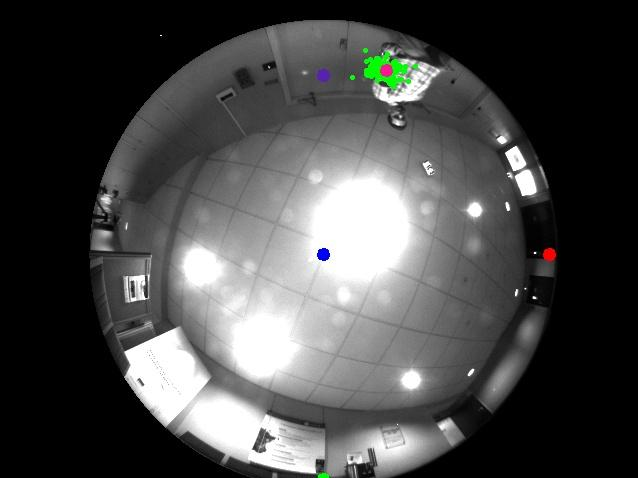
\includegraphics[width=8cm]{images/omnidirectional_camera_markovic.png}
	\end{center}	
	\longcaptionsource{Przykładowy obraz z kamery sferycznej}{}{\cite{Markovic2014}}
\label{fig:Kamera_sferyczna_Markovic}
\end{figure}

Ze względu na rodzaj stosowanego obiektywu konieczne jest przeprowadzenie kalibracji kamery. Polega ona na wyznaczeniu jej wewnętrznego modelu na podstawie którego rejestrowany obraz jest przekształcany w celu usunięcia zniekształceń wnoszonych przez układ optyczny. W pierwszym kroku algorytm wyznacza rzadki przepływ optyczny z wykorzystaniem algorytmu Lucasa-Kanade w wersji piramidowej (rozdział \ref{subsec:Piramidowa_wersja_algorytmu_Lucasa_Kanade}). Następnie wektory przepływu optycznego są rozkładane na składową wynikającą z ruchu robota, wyznaczoną na podstawie odometrii, oraz ewentualną składową wynikającą z ruchu obecnego, poruszającego się obiektu. Zastosowanie kamery sferycznej komplikuje znacznie tą operację, ponieważ manipulowanie punktami obrazu musi odbywać się w przestrzeni współrzędnych sferycznych. Składowe wektorów przepływu optycznego sklasyfikowane jako wynik ruchu obiektów na obrazie są następnie dzielone na grupy, dla których wyznacza się reprezentację pojedynczym wektorem w przestrzeni sferycznej, traktowanym jako wynik pomiarów.

W testowanym rozwiązaniu w przypadku wykrycia wielu obiektów wybierany i śledzony był jedynie najbliższy. Na podstawie wyników pomiarów konstruowany jest probabilistyczny model w postaci rozkładu prawdopodobieństwa von Misesa-Fishera. Właściwe zadanie śledzenia realizowane jest poprzez estymację stanu obiektu z wykorzystaniem rekurencyjnego estymatora Bayesa (którego szczególnym przypadkiem, zakładającym liniowość modelu i rozkłady normalne zmiennych losowych, jest filtr Kalmana opisany w rozdziale \ref{subsec:Klasyczny_filtr_Kalmana}). Finalnie, algorytm śledzenia zwraca estymowany kierunek ruchu obiektu. Na jego podstawie system sterowania wykonuje dodatkowo zadanie utrzymania obiektu w konkretnym, uprzednio zdefiniowanym, obszarze obrazu z kamery. W tym celu estymata kierunku ruchu obiektu jest rzutowana na płaszczyznę obrazu (do współrzędnych sferycznych) i stosowane jest odpowiednie prawo sterowania. 

\section{System wizyjnego śledzenia obiektów w czasie rzeczywistym do zastosowania w wizyjnym serwosterowaniu robota mobilnego}
\label{sec:Przyklad_Zhang2011}

W \cite{Zhang2011} opisany został algorytm śledzenia wizyjnego przeznaczony do zastosowania w systemie sterowania robota mobilnego. Jako założenie projektowe przyjęto odporność na typowe problemy spotykane powiązane ze środowiskiem jego działania (szybki ruch obiektu, przysłonięcia, deformacje, zmiany oświetlenia, mała odrębność tła i obiektu) oraz zdolność wykonania w czasie rzeczywistym. Zwracane przez algorytm położenie obiektu jest przekazywane do systemu sterowania robota. Jako platformę testową wykorzystano robota HBE-RoboCAR-Embedded i jego kamerę pokładową. 

Autorzy publikacji przedstawiają propozycję algorytmu, nazwanego \textit{Modified CamShift Guided Particle Filter} (w skrócie \textit{MCAMSGPF}), integrującego filtr cząsteczkowy z algorytmem \textit{CAMSHIFT} (opisanym w rozdziale \ref{subsec:Algorytm_CAMSHIFT}). Algorytm jest w istocie rozwinięciem koncepcji podobnego rozwiązania o nazwie \textit{CAMSHIFT Guided Particle Filter}, które jednak nie było implementowane w robotyce mobilnej i dlatego nie zostało tutaj przytoczone. Filtr cząsteczkowy (określany inaczej jako sekwencyjna metoda Monte Carlo) jest metodą estymacji stanu, w której rozkład prawdopodobieństwa zmiennych stanu reprezentuje się poprzez zbiór próbek (cząsteczek) z przypisanymi wagami. Każda z cząsteczek reprezentuje możliwy punkt trajektorii stanu, rozkład prawdopodobieństwa jest propagowany w czasie z wykorzystaniem rekursywnego filtru Bayesa, estymacja wartości zmiennych stanu odbywa się poprzez znalezienie w każdym kroku cząsteczki o najwyższej wadze \cite{Chou2012}. Procedura \textit{MCAMSGPF} rozpoczyna się od propagacji poprzedniego, znanego stanu obiektu.
\begin{figure}[!htb]
	\begin{center}
		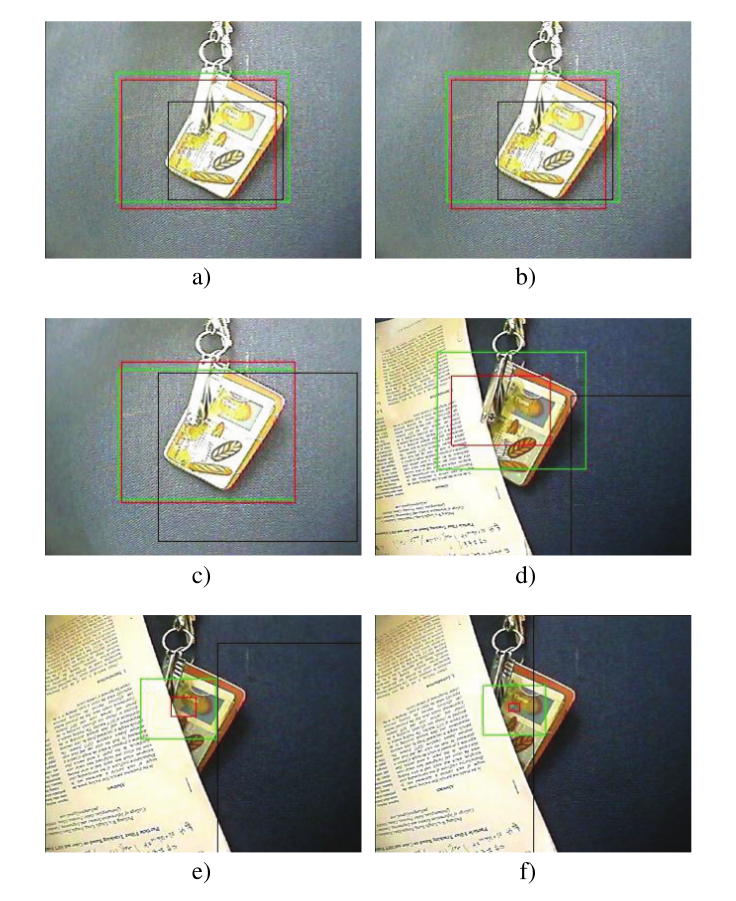
\includegraphics[width=8cm]{images/tracking_example_zhang.png}
	\end{center}	
	\longcaptionsource{Porównanie działania algorytmu \textit{MCAMSGPF} z innymi metodami}{Na obrazach a) - f) przedstawiono klatki wybrane klatki sekwencji video, w której nastąpiło przysłonięcie obiektu zainteresowania. Objaśnienie oznaczeń: zielony prostokąt - obiekt śledzony algorytmem \textit{MCAMSGPF}; czerwony prostokąt - obiekt śledzony algorytmem \textit{CAMSGPF}; obiekt śledzony algorytmem \textit{CAMSHIFT}}{\cite{Zhang2011}}
\label{fig:Przyklad_sledzenia_Zhang}
\end{figure}

Na podstawie założonego dynamicznego modelu w postaci procesu autoregresywnego wyznaczane jest nowe położenie obiektu, które następnie przesuwane jest do minimum lokalnego funkcji gęstości prawdopodobieństwa estymowanej z wykorzystaniem histogramu przestrzeni kolorów \textit{HSV} obrazu. W końcowej fazie propagacji, położenie obiektu (czyli pojedyncza cząsteczka) jest przesuwana na podstawie rozkładu prawdopodobieństwa stanowiącego połączenie rozkładu normalnego z założonym modelem dynamicznym. Na podstawie otrzymanego stanu wykonywany jest model obserwacyjny, oparty o punkty charakterystyczne \textit{SURF} (\textit{Speeded Up Robust Features}). Metoda \textit{SURF} jest modyfikacją metody \textit{SIFT} przytoczonej w rozdziale \ref{subsec:Punkty_charakterystyczne}, której celem było przyspieszenie procesu ekstrakcji i deskrypcji. Punkty \textit{SURF} są inwariantne, co zapewnia odporność całego modelu. Model obserwacyjny służy następnie do określenia wag cząsteczek. Cała przedstawiona wyżej procedura jest wykonywana dla każdej cząsteczki.  Ostatnim krokiem algorytmu jest odrzucenie cząsteczek o zbyt niskich wagach.

Połączenie filtra cząsteczkowego z algorytmem \textit{CAMSHIFT} i modelem opartym o punkty charakterystyczne \textit{SURF} pozwoliło na uzyskanie wysokiej odporności na błędny śledzenia wynikające z przysłonięć obiektu oraz podobieństwa kolorów pikseli tła i obiektu, co jest słabą stroną samej metody \textit{CAMSHIFT} (przykład przedstawiono na rysunku \ref{fig:Przyklad_sledzenia_Zhang}).

\section{System śledzenia obiektów z wykorzystaniem kamery \textit{pan-tilt} zamontowanej na robocie mobilnym}
\label{sec:Przyklad_Kim}

W artykule \cite{Kim2012} zaprezentowano system sterowania głowicą \textit{pan-tilt} z zamontowaną kamerą wizyjną, przeznaczony do zastosowania w robotyce mobilnej, którego funkcją jest utrzymanie obiektu zainteresowania w polu widzenia kamery. W ramach tego zadania estymowane są trójwymiarowe współrzędne obiektu zainteresowania w odniesieniu do lokalnego układu współrzędnych robota oraz obliczane są odpowiednie przemieszczenia kątowe dla silników orientujących kamerę. Zakładany jest ruch robota w przestrzeni trójwymiarowej przy nieruchomym obiekcie zainteresowania.

W przeciwieństwie do innych przykładów rozwiązań przytaczanych w niniejszej pracy, tematyka publikacji \cite{Kim2012} abstrahuje od algorytmów przetwarzania obrazów, skupiając się wyłącznie na systemie sterowania. Zadanie śledzenia obiektu realizowane jest w oparciu o fuzję danych pomiarowych oraz estymację położenia obiektu. Robot stanowiący platformę testową wyposażony jest w enkodery kół, trójosiowy akcelerometr, trójosiowy żyroskop, enkodery silników mechanizmu \textit{pan-tilt} oraz kamerę wizyjną o rozdzielczości $640 \times 480$ pikseli. Do celów testowych, jako obiekt zainteresowania wykorzystywany jest fotografia twarzy, natomiast pomiar polega na wykonaniu odpowiedniego algorytmu wykrywania.
\begin{figure}[!htb]
	\begin{center}
		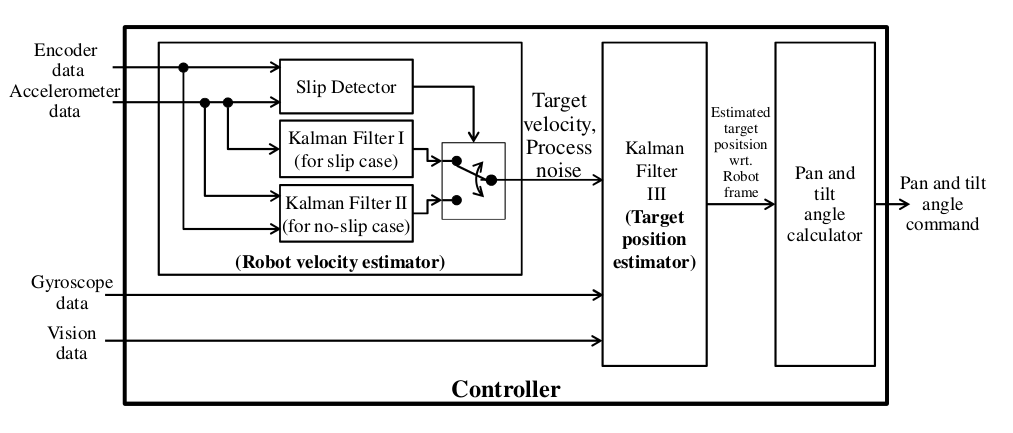
\includegraphics[width=12cm]{images/controller_kim.png}
	\end{center}	
	\longcaptionsource{Schemat systemu sterowania głowicą \textit{pan-tilt}}{}{\cite{Kim2012}}
\label{fig:System_sterowania_Kim}
\end{figure}
System sterowania, którego schemat przedstawia rysunek \ref{fig:System_sterowania_Kim}, składa się z trzech zasadniczych modułów - estymatora prędkości robota, estymatora położenia obiektu zainteresowania i kalkulatora współrzędnych złączowych mechanizmu \textit{pan-tilt}.

Dane wejściowe dla estymatora prędkości stanowią pomiary z enkoderów kół robota oraz akcelerometru. Pomiary wykonywane przy użyciu enkoderów są dokładne, o ile nie występuje utrata przyczepności kół robota (ang. \textit{slip}), w związku z tym są one porównywane ze wskazaniami akcelerometru i w przypadku zbyt dużej rozbieżności stwierdzane jest wystąpienie tego zjawiska. Następnie wybierany jest jeden z dwóch estymatorów prędkości, z których oba mają postać klasycznego filtru Kalmana (opisanego w rozdziale \ref{subsec:Klasyczny_filtr_Kalmana}). Pierwszy z nich, przeznaczony do zastosowania w przypadku wystąpienia utraty przyczepności, estymuje prędkość wyłącznie na podstawie wyników pomiaru akcelerometrem. Drugi, używany przy zachowaniu przyczepności, uwzględnia również pomiary wykonane enkoderami kół, dzięki czemu zapewnia większą dokładność. Moduł estymatora prędkości zwraca pozorną (wynikającą z ruchu robota) prędkość ruchu obiektu zainteresowania w lokalnym układzie współrzędnych robota oraz szum procesu.

Estymator położenia obiektu zainteresowania ma postać rozszerzonego filtru Kalmana (opisanego w rozdziale \ref{subsec:Rozszerzony_filtr_Kalmana}). Poza danymi zwracanymi przez estymator prędkości, wykorzystuje on pomiar wizyjny (położenie obiektu na obrazie z kamery) oraz obecną orientację kamery mierzoną przez żyroskop. Dane wyjściowe stanowi estymowane położenia obiektu zainteresowania w układzie współrzędnych robota, na podstawie który moduł kalkulatora wyznacza wartości współrzędnych złączowych, pozwalające na utrzymanie obiektu zainteresowania w polu widzenia. Częstotliwość próbkowania kamery (27Hz) jest niższa, niż pozostałych sensorów (108Hz). Z tego powodu, pomiędzy kolejnymi klatkami ostatni wyznaczony stan jest propagowany.


\section{Podsumowanie}
\label{sec:Przyklady_podsumowanie}

\todo{Rozszerzyć, krótkie omówienie podejść i algorytmów, mocne/słabe strony, porównanie efektywności algorytmów}

Wśród algorytmów stosowanych w wizyjnym śledzeniu obiektów wyróżnić można dwie grupy:

\begin{enumerate}
	\item Algorytmy tworzące pewną reprezentację obiektu na obrazie i poszukujące jego najbardziej prawdopodobnej instancji na kolejnych klatkach sekwencji video, do których należy algorytm Lucasa-Kanade (\ref{sec:Algorytm_Lucasa_Kanade}) oraz algorytm Mean-Shift (\ref{sec:Algorytm_Mean_Shift}).
	\item Algorytmy dokonujące predykcji trajektorii obiektu na obrazie, do których należą metody oparte o rekursywny filtr Bayesa, tj. filtr Kalmana (\ref{sec:Filtr_Kalmana}) i filtr cząsteczkowy
\end{enumerate}

Pomimo pozornie różnych funkcji, obie grupy mogą stanowić źródło sprzężenia zwrotnego dla systemu sterowania robota mobilnego. Zaznaczyć należy, że zastosowanie algorytmów z grupy drugiej wymaga wdrożenia dodatkowego mechanizmu  pomiaru położenia obiektu, np. poprzez okresowe wykonanie procedury wykrywania go na podstawie wzorca.

Obszar aplikacji w postaci robotyki mobilnej dodatkowo utrudnia nietrywialne z natury zadanie śledzenia obiektów. Poza ruchem samego obiektu należy brać pod uwagę możliwość ruchu samego robota, skutkującą zwiększeniem częstości występowania niepożądanych zjawisk, takich jak przysłonięcia obiektu zainteresowania, zmiany oświetlenia sceny czy niewielka rozbieżność pomiędzy wyglądem obiektu zainteresowania a tłem. Dodatkowo, ruch kamery zmienia wynik działania niektórych powszechnie stosowanych metod, np. w polu przepływu optycznego pojawia się składowa stała, reprezentująca pozorny ruch całej sceny. W przypadku platformy sprzętowej w postaci robota mobilnego często należy liczyć się z jej niewielką wydajnością obliczeniową.

W celu zwiększenia ogólnej odporności systemu śledzenia, częstym rozwiązaniem jest wykorzystanie więcej niż jednego algorytmu śledzenia wizyjnego (\cite{Liem2008}, \cite{Zhang2011}, \cite{Markovic2014}). W takich przypadkach dane zwracane przez pierwszy stanowią dane wejściowe kolejnego, co pozwala na wzajemną kompensację nieprawidłowego działania.

Standardowym typem stosowanego czujnika wizyjnego jest pojedyncza kamera video o niskiej rozdzielczości (\cite{Liem2008}, \cite{Olivares-Mendez2009}, \cite{Zhang2011}, \cite{Kim2011}, wyjątek stanowi \cite{Markovic2014}). Jest to zrozumiałe, ze względu na wspomniane wcześniej ograniczenie mocy obliczeniowej, istotne w przypadku komputerów pokładowych.

